\documentclass[tikz,border=10pt]{standalone}
\usepackage{tkz-euclide} % 辅助几何图形绘制

\begin{document}
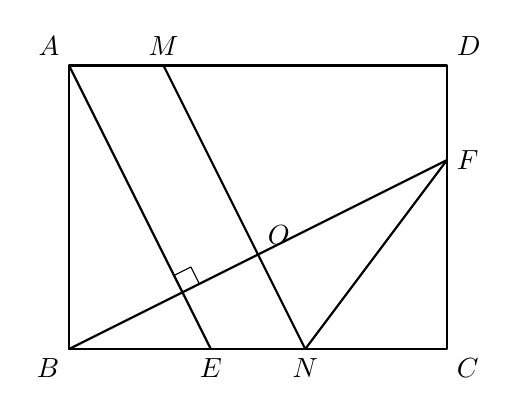
\begin{tikzpicture}[scale=1.2, line cap=round, line join=round]
    % 1. 定义矩形的四个顶点 (假设长宽比约为 4:3)
    \coordinate (B) at (0,0);
    \coordinate (C) at (4,0);
    \coordinate (D) at (4,3);
    \coordinate (A) at (0,3);

    % 2. 定义关键点坐标 (根据图像比例估算)
    \coordinate (E) at (1.5,0);     % 边 BC 上的点 E
    \coordinate (F) at (4,2);     % 边 CD 上的点 F
    \coordinate (M) at (1,3);       % 边 AD 上的点 M
    \coordinate (N) at (2.5,0);     % 边 BC 上的点 N

    % 3. 计算交点
    % O 为 MN 与 BF 的交点
    \coordinate (O) at (intersection of M--N and B--F);

    % 4. 绘制主要几何轮廓
    \draw[thick] (A) -- (B) -- (C) -- (D) -- cycle; % 矩形 ABCD
    \draw[thick] (A) -- (E);                        % 线段 AE
    \draw[thick] (B) -- (F);                        % 线段 BF
    \draw[thick] (M) -- (N);                        % 线段 MN
    \draw[thick] (N) -- (F);                        % 线段 NF

    % 5. 标注垂直符号 (AE 垂直于 BF)
    % 寻找 AE 与 BF 的交点用于绘制直角符号
    \coordinate (P) at (intersection of A--E and B--F);
    \tkzMarkRightAngle[size=0.2](A,P,F);

    % 6. 标记所有点名称
    \node[above left]  at (A) {$A$};
    \node[below left]  at (B) {$B$};
    \node[below right] at (C) {$C$};
    \node[above right] at (D) {$D$};
    \node[above]       at (M) {$M$};
    \node[below]       at (N) {$N$};
    \node[below]       at (E) {$E$};
    \node[right]       at (F) {$F$};
    \node[above right] at (O) {$O$};

\end{tikzpicture}
\end{document}